\thispagestyle{cackithitoannone}
\pagestyle{cackithitoan}
\everymath{\color{cackithi}}
\graphicspath{{../cackithi/pic/}}
\begingroup
\AddToShipoutPicture*{\put(0,616){\includegraphics[width=19.3cm]{../bannercackithi}}}
\AddToShipoutPicture*{\put(78,523){\includegraphics[scale=1]{../tieude.pdf}}}
\centering
\endgroup
\vspace*{180pt}

\begin{multicols}{2}
	Câu lạc bộ Unicorn Math Circle -- UMC được Tạp chí Pi tổ chức từ năm $2019$ với sự hỗ trợ của Viện Toán học. Bắt đầu từ năm học $2022-2023$, các lớp CLB mới của UMC sẽ hoạt động trong khuôn khổ hợp tác giữa Tạp chí Pi và Minh Việt Academy -- MVA.
	\vskip 0.1cm
	UMC là một câu lạc bộ toán học dành cho học sinh Tiểu học và THCS nhằm tìm kiếm và bồi dưỡng các học sinh có năng lực Toán học. CLB sẽ tập trung phát triển năng lực suy nghĩ và sự sáng tạo của các bạn trẻ thông qua các chuyên đề Toán học.
	\vskip 0.1cm
	Hoạt động như một tổ chức phi lợi nhuận, UMC luôn là địa chỉ để đón chào các bạn nhỏ có năng khiếu toán trên mọi miền tổ quốc, kể cả nước ngoài, các bạn khó khăn sẽ được xét để cấp học bổng. Xin mời các bạn thử sức với một số bài tập trong kỳ thi chọn của UMC năm $2020$. (Đáp số ở cuối bài). 
	\vskip 0.1cm
	\textbf{\color{cackithi}Bài} $\pmb{1.}$ Các con búp bê Nga (có tên là Matryoshka) có chiều cao lần lượt là: $32$, $40$, $52$, $68$, $88$, $112$ và $140$ mm.
	\begin{figure}[H]
		\centering
		\vspace*{-10pt}
		\captionsetup{labelformat= empty, justification=centering}
		\includegraphics[width=0.85\linewidth]{Bai1}
		\vspace*{-5pt}
	\end{figure}
	Bạn hãy tính xem tổng chiều cao của các con búp bê này bằng bao nhiêu mm.
	\vskip 0.1cm
	\textbf{\color{cackithi}Bài} $\pmb{2.}$ Bạn An muốn làm tăng chu vi của hình bên bằng cách xóa đi $1$ ô vuông nhỏ. Hỏi bạn An cần xóa đi ô vuông nào?
	\begin{figure}[H]
		\centering
		\vspace*{-5pt}
		\captionsetup{labelformat= empty, justification=centering}
		\begin{tikzpicture}[cackithi]
			\draw (0,0) grid (5,1);
			\draw (1,-1) grid (6,0);
			\draw (1,-2) grid (3,-1);
			\draw (0.5,0.5) node{$A$};
			\draw (1.5,0.5) node{$B$};
			\draw (2.5,0.5) node{$C$};
			\draw (3.5,0.5) node{$D$};
			\draw (4.5,0.5) node{$E$};
			\draw (1.5,-0.5) node{$F$};
			\draw (2.5,-0.5) node{$G$};
			\draw (3.5,-0.5) node{$H$};
			\draw (4.5,-0.5) node{$I$};
			\draw (5.5,-0.5) node{$J$};
			\draw (1.5,-1.5) node{$K$};
			\draw (2.5,-1.5) node{$L$};
		\end{tikzpicture}
		\vspace*{-10pt}
	\end{figure}	 
	\textbf{\color{cackithi}Bài} $\pmb{3.}$ Hai hình $ABCDEF$ và $UVWXYZ$ giống hệt nhau về kích thước và hình dáng. Đố bạn biết cạnh nào của hình $UVWXYZ$ có độ dài bằng cạnh $DE$?
	\begin{figure}[H]
		\centering
		\vspace*{-5pt}
		\captionsetup{labelformat= empty, justification=centering}
		\includegraphics[width=1\linewidth]{Bai2}
		\vspace*{-10pt}
	\end{figure}
	\textbf{\color{cackithi}Bài} $\pmb{4.}$ Tháp gỗ sau được xếp bằng các viên gỗ nhỏ hình lập phương, viên này chồng lên viên kia. Có một số viên gỗ không nhìn thấy được.
	\vskip 0.1cm
	Hỏi số viên gỗ không nhìn thấy được nhiều hơn số viên gỗ nhìn thấy được là bao nhiêu viên?
	\begin{figure}[H]
		\centering
		\vspace*{-5pt}
		\captionsetup{labelformat= empty, justification=centering}
		\includegraphics[width=0.7\linewidth]{Bai4}
		\vspace*{-10pt}
	\end{figure}
	\textbf{\color{cackithi}Bài} $\pmb{5.}$ Hình chữ nhật sau được chia thành bốn hình tam giác có diện tích là $2$, $3$, $5$ và $x$ như hình vẽ.
	\begin{figure}[H]
		\centering
		\vspace*{-5pt}
		\captionsetup{labelformat= empty, justification=centering}
		\begin{tikzpicture}[cackithi,scale=0.85]
			\fill[fill=cackithi,fill opacity=0.10000000149011612] (0,3) -- (2,2) -- (5,3) -- cycle;
			\fill[fill=toanhocdoisong,fill opacity=0.10000000149011612] (0,0) -- (2,2) -- (5,0) -- cycle;
			\draw  (0,0)-- (0,3);
			\draw  (0,3)-- (5,3);
			\draw  (5,3)-- (5,0);
			\draw  (5,0)-- (0,0);
			\draw  (0,3)-- (2,2);
			\draw  (2,2)-- (5,3);
			\draw  (5,3)-- (0,3);
			\draw  (0,0)-- (2,2);
			\draw  (2,2)-- (5,0);
			\draw  (5,0)-- (0,0);
			\draw (0.7715297724476833,1.9968077986358754) node {$3$};
			\draw (3.9949386709976675,1.8798965950615238) node {$x$};
			\draw (2.1911658158505265,2.698275020081985) node {$2$};
			\draw (2.2245690168717696,1.0448165695304408) node {$5$};
		\end{tikzpicture}
		\vspace*{-10pt}
	\end{figure}
	Tính giá trị của $x$?
	\vskip 0.1cm 	 
	\textbf{\color{cackithi}Bài} $\pmb{6.}$ Hình sau có bao nhiêu hình tam giác?
	\begin{figure}[H]
		\centering
		\vspace*{-5pt}
		\captionsetup{labelformat= empty, justification=centering}
		\begin{tikzpicture}[cackithi,scale=0.85]
			\draw  (0,0)-- (4.529389887337568,0);
			\draw  (4.529389887337568,0)-- (2.2646949436687853,3.922566706078671);
			\draw  (2.2646949436687853,3.922566706078671)-- (0,0);
			\draw  (0.8383361744901764,0)-- (4.529389887337568,0);
			\draw  (4.529389887337568,0)-- (2.683863030913873,3.196546282058714);
			\draw  (2.683863030913873,3.196546282058714)-- (0.8383361744901764,0);
			\draw  (0,0)-- (3.59696996366193,0);
			\draw  (3.59696996366193,0)-- (1.7984849818309656,3.115067365180821);
			\draw  (1.7984849818309656,3.115067365180821)-- (0,0);
			\draw  (0,0)-- (4.050858326392901,0);
			\draw  (4.050858326392901,0)-- (2.0254291631964514,3.508146217787968);
			\draw  (2.0254291631964514,3.508146217787968)-- (0,0);
			\draw  (0.9396160733024788,1.6274627785682547)-- (3.5936444563102365,1.6207586294897776);
			\draw  (0.7047120549768591,1.220597083926191)-- (3.827580814067069,1.215568972117333);
			\draw  (0.4698080366512394,0.8137313892841274)-- (4.061517171823902,0.8103793147448888);
			\draw  (0.2349040183256197,0.4068656946420637)-- (4.295453529580735,0.4051896573724444);
		\end{tikzpicture}
		\vspace*{-10pt}
	\end{figure}
	\textbf{\color{cackithi}Bài} $\pmb{7.}$ Các ô vuông của hình sau được điền các số tự nhiên khác $0$ sao cho trên mỗi hàng là các số khác nhau, và số nằm ở ô vuông bên trên bằng tích của hai số được ghi ở hai ô vuông nằm bên dưới nó.
	\begin{figure}[H]
		\centering
		\vspace*{-5pt}
		\captionsetup{labelformat= empty, justification=centering}
		\begin{tikzpicture}[cackithi,scale=0.85]
			\draw (0,0) grid (3,1);
			\draw (1,2) grid (2,3);
			\draw (0.5,1) rectangle (2.5,2);
			\draw (1.5,1) -- (1.5,2);
			\draw (1.5,2.5) node{$X$};
		\end{tikzpicture}
		\vspace*{-10pt}
	\end{figure}
	Hỏi $X$ có giá trị nhỏ nhất bằng bao nhiêu?
	\vskip 0.1cm	
	\textbf{\color{cackithi}Bài} $\pmb{8.}$ Cho $8$ điểm nằm trên một lưới ô vuông như hình vẽ. Hỏi có bao nhiêu tam giác có các đỉnh là $3$ trong số $8$ điểm đã cho.
	\begin{figure}[H]
		\centering
		\vspace*{-5pt}
		\captionsetup{labelformat= empty, justification=centering}
		\begin{tikzpicture}
			\fill[cackithi] (0,0) circle (2.5pt);
			\fill[cackithi] (0,1) circle (2.5pt);
			\fill[cackithi] (1,0) circle (2.5pt);
			\fill[cackithi] (1,1) circle (2.5pt);
			\fill[cackithi] (0,2) circle (2.5pt);
			\fill[cackithi] (2,0) circle (2.5pt);
			\fill[cackithi] (1,2) circle (2.5pt);
			\fill[cackithi] (2,2) circle (2.5pt);
		\end{tikzpicture}
		\vspace*{-10pt}
	\end{figure}
	\textbf{\color{cackithi}Bài} $\pmb{9.}$ Trên bảng ghi $9$ số $1,2,3,4,\ldots,9$. Bạn Nam muốn chọn ra một số số có tổng bằng $32$. Hỏi bạn Nam cần chọn ra ít nhất bao nhiêu số?
	\vskip 0.1cm
	\textbf{\color{cackithi}Bài} $\pmb{10.}$ Việt có $3$ chìa khóa để mở $3$ ổ khóa bên ngoài một chiếc hòm đựng báu vật, mỗi chìa chỉ mở được đúng $1$ ổ khóa. Tuy nhiên Việt không nhớ chìa nào ứng với ổ khóa nào. Hỏi Việt phải  tra chìa vào ổ khóa để thử ít nhất mấy lần để chắc chắn xác định được chìa khóa nào là của ổ khóa nào.
	\vskip 0.1cm
	\textbf{\color{cackithi}Bài} $\pmb{11.}$ Điền số thích hợp vào chỗ trống:
	\begin{align*}
		261, 220, 202, 612, 202, 026, \_\_\_
	\end{align*}
	\textbf{\color{cackithi}Bài} $\pmb{12.}$ Biết rằng tổng các chữ số của một số tự nhiên có $3$ chữ số bằng $7$. Liệt kê tất cả các giá trị có thể của tổng các chữ số của số liền trước nó? 
	\vskip 0.1cm
	\textbf{\color{cackithi}Bài} $\pmb{13.}$ Ngày $26$ tháng $12$ năm $2020$ là ngày thứ bảy. Hỏi ngày này sau đúng $60$ năm sau ($26/12/2080$) là thứ mấy?
	\vskip 0.1cm
	\textbf{\color{cackithi}Bài} $\pmb{14.}$ Có bao nhiêu số có $3$ chữ số mà chữ số hàng trăm lớn hơn chữ số hàng đơn vị.
	\vskip 0.1cm
	\textbf{\color{cackithi}Bài} $\pmb{15.}$ Có bao nhiêu cách lát kín một mảnh đất hình chữ nhật kích thước $5(m)\times2(m)$ bằng các tấm bê tông hình chữ nhật kích thước $1(m)\times2(m)$.
	\vskip 0.1cm
	\textbf{\color{cackithi}Bài} $\pmb{16.}$ Điền số thích hợp vào chỗ trống:
	\begin{align*}
		6, 12, 15, 21, 24, 30, \_\_\_
	\end{align*}
	\vskip 0.1cm
	Bài $17$. Có bao nhiêu cách để chia $4$ bạn Đông, Tây, Nam, Bắc thành hai nhóm, mỗi nhóm có $2$ bạn?
	\vskip 0.1cm
	\textbf{\color{cackithi}Bài} $\pmb{18.}$ Có bao nhiêu số điện tử có $3$ chữ số (digital number) mà giá trị của nó không đổi khi ta nhìn trong gương? (số có $3$ chữ số này có chữ số hàng trăm khác $0$).
	\vskip 0.1cm
	\textit{Chữ số điện tử:} 
	\begin{figure}[H]
		\centering
		\vspace*{-10pt}
		\captionsetup{labelformat= empty, justification=centering}
		\includegraphics[width=1\linewidth]{Bai18}
		\vspace*{-15pt}
	\end{figure}
	\textbf{\color{cackithi}Bài} $\pmb{19.}$ Trên bảng ta vẽ $5$ đường tròn (không có hai đường tròn nào trùng nhau), hỏi $5$ đường tròn này cắt nhau tại nhiều nhất bao nhiêu điểm? 
	\vskip 0.1cm
	\textbf{\color{cackithi}Bài} $\pmb{20.}$ Có bao nhiêu số có ba chữ số chia hết cho $3$ mà không chứa chữ số $3$?
	\vskip 0.1cm
	\textbf{\color{cackithi}Lời giải, đáp án}
	\vskip 0.1cm
	\textbf{\color{cackithi}Bài} $\pmb{1.}$ Đáp số: $32+40+52+68+88+112=392$ $(mm)$.
	\vskip 0.1cm
	\textbf{\color{cackithi}Bài} $\pmb{2.}$ Đáp số: $G$.
	\vskip 0.1cm
	\textbf{\color{cackithi}Bài} $\pmb{3.}$ Đáp số: $UV$.	 
	\vskip 0.1cm
	\textbf{\color{cackithi}Bài} $\pmb{4.}$
	\textit{Lời giải} $1$.
	Tổng số viên: $1\times5+2\times4+3\times3+4\times2+5 = 35$.
	\vskip 0.1cm
	Số viên nhìn thấy: $1+2+3+4+5 = 15$.
	\vskip 0.1cm
	Số viên không nhìn thấy: $35 - 15 = 20$.
	\vskip 0.1cm
	Đáp số: $20 - 15 = 5$.
	\vskip 0.1cm
	\textit{Lời giải} $2$.
	Số viên nhìn thấy: $1+2+3+4+5 = 15$.
	\vskip 0.1cm
	Số viên không nhìn thấy: $4 + 3\times2 + 2\times3 + 1\times4 = 20$.
	\vskip 0.1cm
	Đáp số: $20 - 15 = 5$.
	\vskip 0.1cm
	\textbf{\color{cackithi}Bài} $\pmb{5.}$ \textit{Lời giải}.
	Hai tam giác Xanh, Đỏ có đáy bằng nhau bằng chiều dài hình chữ nhật, tổng chiều cao bằng chiều rộng hình chữ nhật $\Rightarrow$ Tổng diện tích bằng một nữa hình chữ nhật. Vậy ta có:
	\begin{align*}
			2 + 5 = 3 + X \Rightarrow X = 4.
		\end{align*}
	Đáp số: $4$.
	\vskip 0.1cm
	\textbf{\color{cackithi}Bài} $\pmb{6.}$ \textit{Lời giải}.
	Như trên hình vẽ, mỗi tam giác có đáy, cạnh bên trái và cạnh bên phải.
	\vskip 0.1cm
	Chọn đáy: $5$ (cách).
	\vskip 0.1cm
	Chọn cạnh bên phải: $3$ (cách). 
	\vskip 0.1cm
	Chọn cạnh bên trái: $2$ (cách).
	\vskip 0.1cm
	Theo quy tắc nhân, số tam giác là: $5\times3\times2 = 30$.
	\vskip 0.1cm
	Đáp số: $30$.
	\vskip 0.1cm
	\textbf{\color{cackithi}Bài} $\pmb{7.}$ \textit{Lời giải}.
	\begin{figure}[H]
		\centering
		\vspace*{-5pt}
		\captionsetup{labelformat= empty, justification=centering}
		\begin{tikzpicture}[cackithi, scale=0.85]
				\draw (0,0) grid (3,1);
		\draw (1,2) grid (2,3);
		\draw (0.5,1) rectangle (2.5,2);
		\draw (1.5,1) -- (1.5,2);
		\draw (1.5,2.5) node{$X$};
		\draw(0.5,0.5) node{$a$};
		\draw(1.5,0.5) node{$b$};
		\draw(2.5,0.5) node{$c$};
		\draw(1,1.5) node{$ab$};
		\draw(2,1.5) node{$bc$};
		\end{tikzpicture}
		\vspace*{-10pt}
	\end{figure}
	Gọi $3$ số hàng cuối là $a,b,c$ ($a\ne b\ne c > 0$).
	\vskip 0.1cm
	Hàng $2$ có $2$ số là: $ab$ và $bc$.
	\vskip 0.1cm
	Vậy $X = ab\times bc = ab^2c$ bé nhất khi $b=1$, $a=2$, $c=3$ hoặc $b=1$, $a=3$, $c=2$.
	\vskip 0.1cm
	Vậy giá trị nhỏ nhất của $X$ là: $2\times 1^2\times3 = 6$.
	\vskip 0.1cm
	Đáp số: $6$
	\vskip 0.1cm
	\textbf{\color{cackithi}Bài} $\pmb{8.}$ \textit{Lời giải}.
	Số cách chọn $3$ điểm: 
	\begin{align*}
			C_8^3 = \frac{8\times 7 \times 6}{3!} = 56.
		\end{align*}
	Số tam giác suy biến (tam giác có $3$ điểm thẳng hàng): $6$.
	\vskip 0.1cm
	Số tam giác là: $56 - 6 = 50$.
	\vskip 0.1cm
	\textbf{\color{cackithi}Bài} $\pmb{9.}$ \textit{Lời giải}. 
	Để chọn ít nhất Nam cần rút những số lớn nhất có thể.
	\vskip 0.1cm
	$32 = 9 + 8 + 7 + 6 + 2$. Vậy Nam cần chọn $5$ số $(9,8,7,6,2)$.
	\vskip 0.1cm
	Đáp số: $5$.
	\vskip 0.1cm
	\textbf{\color{cackithi}Bài} $\pmb{10.}$ \textit{Lời giải}.
	Thử chìa đầu tiên: $2$ lần thử thì xác định được sẽ mở ổ nào (Nếu $2$ lần thử không được thì chìa sẽ mở được ổ còn lại).
	\vskip 0.1cm
	Thử chìa $2$: $1$ lần sẽ xác định được mở ổ nào.
	\vskip 0.1cm
	Chìa còn lại sẽ mở được ổ còn lại. Vậy số lần thử ít nhất là: $2+1=3$.
	\vskip 0.1cm
	Đáp số: $3$.
	\vskip 0.1cm
	\textbf{\color{cackithi}Bài} $\pmb{11.}$ \textit{Lời giải}.
	$2612202026122020\ldots$ nó chính là dãy $26/12/2020$ lặp đi lặp lại.
	\vskip 0.1cm
	Vậy số tiếp theo là $122$.
	\vskip 0.1cm
	Đáp số: $122$.
	\vskip 0.1cm
	\textbf{\color{cackithi}Bài} $\pmb{12.}$. \textit{Lời giải} $1$.
	Nếu số đó là $700$. Số liền trước là $699$ có tổng các chữ số bằng $6+9+9=24$.
	\vskip 0.1cm
	Nếu số đó là: $\overline{ab0}$ ($b\ne0$), số liền trước là: $\overline{(a(b-1)9)}$ có tổng các chữ số 
	bằng
	\begin{align*}
			a+b-1+9=a+b+8=7+8=15.
		\end{align*}
	Nếu số đó là $\overline{abc}$ ($c\ne0$), số liền trước là: $\overline{ab(c-1)}$ có tổng các chữ số bằng
	\begin{align*}
			a+b+c-1=7-1=6.
		\end{align*}
	Vậy các giá trị có thể của tổng các chữ số liền trước là: $\{6,15,24\}$.
	\vskip 0.1cm 
	\textit{Lời giải} $2$.
	Số có $3$ chữ số có tổng các chữ số bằng $7$ chia $9$ dư $7$. Vậy số liền trước là số có $3$ chữ số chia $9$ dư $6$. Vậy tổng các chữ số của nó có thể nhận các giá trị $\{6,15,24\}$ (do $9\times 3 = 27 < 33$). Thử với $3$ số $115$, $160$, $700$ có các số liền trước là $114$, $159$, $699$ có tổng các chữ số tương ứng là $6$, $15$, $24$.
	\vskip 0.1cm
	\textit{Lời giải} $3$. Liệt kê các số có $3$ chữ số thỏa mãn là $106$, $115$, $124$, $133$, $142$, $151$, $160$, $205$, $214$, $223$, $232$, $241$, $250$, $304$, $313$, $322$, $331$, $340$, $403$, $412$, $421$, $430$, $502$, $511$, $520$, $601$, $610$, $700$.
	\vskip 0.1cm
	Số liền trước: $105\ldots$, $159$, $249$, $339$, $429$, $519$, $609$, $699$ có tổng các chữ số là: $6$, $15$, $24$.
	\vskip 0.1cm
	Đáp số: $6$, $15$, $24$.
	\vskip 0.1cm
	\textbf{\color{cackithi}Bài} $\pmb{13.}$ \textit{Lời giải}.
	Năm thường có $365$ ngày chia $7$ dư $1$ $\Rightarrow$ $60\times 365$ chia $7$ dư $4$.
	\vskip 0.1cm
	$60$ năm có $60:4=15$ năm nhuận, thêm $15$ ngày, chia $7$ dư $1$.
	\vskip 0.1cm
	Vậy số ngày trong $60$ năm chia $7$ dư $5$, vậy sau $5$ ngày từ thứ $7$ là thứ $5$.
	\vskip 0.1cm
	Đáp số: Thứ $5$.
	\vskip 0.1cm
	\textbf{\color{cackithi}Bài} $\pmb{14.}$ \textit{Lời giải}.
	Gọi số đó là $\overline{abc}$.
	\vskip 0.1cm
	+ $b$ có $10$ cách chọn.
	\vskip 0.1cm
	+ $\overline{ac}$ có số cách chọn là: $1+2+3+\ldots+9 = 45$ (Hoặc mỗi cặp $2$ chữ số có đúng $1$ số $\overline{ac}$ thỏa mãn $a>c$ nên số cách chọn $\overline{ac}$ là: $C^2_{10} = 45$).
	\vskip 0.1cm
	Vậy số số có $3$ chữ số thỏa mãn là: $10\times45=450$.
	\vskip 0.1cm
	Đáp số: $450$ .
	\vskip 0.1cm
	\textbf{\color{cackithi}Bài} $\pmb{15.}$ \textit{Hướng dẫn giải}.
	Số cách lát hình chữ nhật $k(m) \times 2(m)$ bằng các viên gạch $1(m)\times2(m)$ chính là dãy Fibonacci $1,2,3,5,8,\ldots$. Vậy số cách lát là: $F5 = 8$.
	\vskip 0.1cm
	Đáp số: $8$.
	\vskip 0.1cm
	\textbf{\color{cackithi}Bài} $\pmb{16.}$ Đáp số: $33$.
	\vskip 0.1cm 
	\textbf{\color{cackithi}Bài} $\pmb{17.}$ \textit{Lời giải}. Đông có thể ghép cặp với Tây, Nam hoặc Bắc. Vậy có $3$ cách chia nhóm.
	\vskip 0.1cm
	Đáp số: $3$.
	\vskip 0.1cm
	\textbf{\color{cackithi}Bài} $\pmb{18.}$ \textit{Lời giải}.
	Gọi số có $3$ chữ số là: $\overline{abc}$.
	\vskip 0.1cm
	+ Số cách chọn $b$ là $3$ $(0,1,8)$.
	\vskip 0.1cm
	+ Số cách chọn $\overline{ac}$ là: $4$ $(11, 88,25, 52)$.
	\vskip 0.1cm
	Đáp số: $3\times 4=12$.
	\vskip 0.1cm
	\textbf{\color{cackithi}Bài} $\pmb{19.}$ \textit{Lời giải}. Số điểm cắt nhiều nhất xảy ra khi hai đường tròn bất kỳ đều cắt nhau tại $2$ điểm và không có $3$ đường tròn nào cắt nhau tại $1$ điểm. Khi đó mỗi đường tròn cắt $4$ đường tròn kia tại $4\times 2=8$ điểm $\Rightarrow$ Số điểm cắt sẽ là: $8\times 5 = 40$, tuy nhiên mỗi điểm sẽ được tính $2$ lần (vì đường tròn $A$ cắt $B$ tại $2$ điểm chính là $2$ điểm của đường tròn $B$ cắt $A$). Vậy số điểm cắt nhiều nhất của $5$ đường tròn là: $40:2 = 20$.
	\vskip 0.1cm
	Đáp số: $20$ (điểm).
	\vskip 0.1cm
	\textbf{\color{cackithi}Bài} $\pmb{20.}$ \textit{Lời giải}. 
	Gọi số đó là $\overline{abc}$.
	\vskip 0.1cm
	Nếu $\overline{ab}$ chia $3$ dư $0$: $c\in \{0,6,9\}$ -- có $3$ cách chọn $c$.
	\vskip 0.1cm  
	Nếu $\overline{ab}$ chia $3$ dư $1$: $c\in \{2,5,8\}$ -- có $3$ cách chọn $c$.
	\vskip 0.1cm  
	Nếu $\overline{ab}$ chia $3$ dư $2$: $c\in \{1,4,7\}$ -- có $3$ cách chọn $c$.
	\vskip 0.1cm  
	Vậy với mỗi số $\overline{ab}$ đều có $3$ cách chọn $c$. Số các số có $2$ chữ số đều khác $3$ là: $8\times9=72$.
	\vskip 0.1cm
	Số số có $3$ chữ số thỏa mãn là: $72\times 3=216$.
	\vskip 0.1cm
	Đáp số: $216$. 
\end{multicols}
\newpage
\begingroup
\AddToShipoutPicture*{\put(150,695){\includegraphics[scale=1]{../tieude1.pdf}}}
\centering
\endgroup
\vspace*{10pt}
\begin{multicols}{2}
	Trong phần đầu chuyên mục, chúng tôi sẽ trình bày \textit{Lời giải} của các bài toán trong kỳ thi  Olympic Toán học Trẻ của Canada năm học $2022$  đăng trong số báo $11/2022$. 
	\begin{figure}[H]
		\centering
		\vspace*{-5pt}
		\captionsetup{labelformat= empty, justification=centering}
		\includegraphics[width=1\linewidth]{gocolympic}
		\vspace*{-10pt}
	\end{figure}
	{\bf\color{cackithi} OC$\pmb{25.}$} Cho $ABC$ là tam giác nhọn nội tiếp đường tròn $\Gamma.$ Đường thẳng qua $A$ vuông góc với $BC$ cắt $\Gamma$ tại $D,$ và đường thẳng qua $B$ vuông góc với $AC$ cắt $\Gamma$ tại $E.$ Chứng minh rằng nếu $AB = DE$, thì $\angle ACB = 60^{\circ}.$
	\vskip 0.1cm
	\textit{\textit{Lời giải}.} 
	\begin{figure}[H]
		\vspace*{-5pt}
		\centering
		\captionsetup{labelformat= empty, justification=centering}
		\begin{tikzpicture}[cackithi]
			\draw (0.9004185552987112,2.2669457035324743) -- (1.0180882363816217,2.0904411819081083) -- (1.1945927580059874,2.208110862991019) -- (1.0769230769230769,2.3846153846153846) -- cycle; 
			\draw (-0.4987538820250189,1.8329179606750063) -- (-0.4316718427000252,2.0341640786499875) -- (-0.6329179606750064,2.101246117974981) -- (-0.7,1.9) -- cycle; 
			\draw  (0.5,2.1666666666666665) circle (1.9002923751652299cm);
			\draw  (-1.,1.)-- (2.,1.);
			\draw  (2.,1.)-- (0.,4.);
			\draw  (0.,4.)-- (-1.,1.);
			\draw  (-1.,1.)-- (2.1538461538461533,3.102564102564102);
			\draw  (2.,1.)-- (-1.4,2.1333333333333333);
			\draw  (-1.4,2.1333333333333333)-- (2.1538461538461533,3.102564102564102);
			\draw  (2.1538461538461533,3.102564102564102)-- (0.,4.);
			\draw  (0.,4.)-- (-1.4,2.1333333333333333);
				\draw [fill=white] (-1.,1.) circle (1.5pt);
				\draw (-1.3,0.79) node {$A$};
				\draw [fill=white] (2.,1.) circle (1.5pt);
				\draw (2.3,0.77) node {$B$};
				\draw [fill=white] (0.,4.) circle (1.5pt);
				\draw (0.,4.45) node {$C$};
				\draw [fill=white] (2.1538461538461533,3.102564102564102) circle (1.5pt);
				\draw (2.36,3.49) node {$D$};
				\draw [fill=white] (-1.4,2.1333333333333333) circle (1.5pt);
				\draw (-1.7,2.21) node {$E$};
		\end{tikzpicture}
		\vspace*{-10pt}
	\end{figure}
	Do $ABC$ là tam giác nhọn nên các điểm $D$ và $E$ lần lượt nằm ở bên trong cung nhỏ $BC$ và $AC$ như trong hình vẽ. Như vậy $\angle ECD$ lớn hơn  $\angle ACB$. Từ giả thiết $AB=DE,$ ta có $\angle ECD= 180^\circ - \angle ACB$.  \hfill ($1$)
	\vskip 0.1cm
	Mặt khác ta có
	\begin{align*}
		\angle ECD =\,&\angle ECA + \angle ACB + \angle BCD \\
		= \,&\angle EBA + \angle ACB + \angle BAD \\
		= \,&90^\circ \!\!-\!\! \angle BAC \!\!+\!\! \angle ACB \!\!+\!\! 90^\circ \!\!-\!\! \angle ABC \\
		= \,&(180^\circ \!-\! \angle BAC \!-\! \angle ABC) \!+\! \angle ACB  \\
		= \,&2\angle ACB  \tag{$2$}
	\end{align*}
	Từ ($1$) và ($2$) ta nhận được điều cần chứng minh.
	\vskip 0.1cm
	{\bf\color{cackithi} OC$\pmb{26.}$} Giả sử bạn có vô hạn các hình chữ $T$ (bao gồm bốn hình vuông cạnh
	$1$) như trong hình vẽ, và một bảng ô vuông cỡ $n \times n.$ Bạn được phép đặt một số hình trên bảng (có thể xoay chúng), miễn là không có hai hình nào chồng lên nhau và không có hình nào vượt ra khỏi bảng.
	\vskip 0.1cm
	Với những giá trị nào của $n$ thì bạn có thể phủ toàn bộ bảng?
	\begin{figure}[H]
		\vspace*{-5pt}
		\centering
		\captionsetup{labelformat= empty, justification=centering}
		\begin{tikzpicture}[cackithi,scale=0.88]
			\draw (0,0) grid (3,1);
			\draw (1,-1) grid (2,0);
		\end{tikzpicture}
		\vspace*{-10pt}
	\end{figure}
	\textit{\textit{Lời giải}.} Trước tiên ta nhận thấy mỗi hình chữ $T$ gồm $4$ ô, do đó nếu phủ kín được bảng thì diện tích của bảng phải chia hết cho $4$, tức là $n$ chẵn.
	\vskip 0.1cm
	Với $n$ chia hết cho $4$ ta có thể chia bảng thành các bảng con cỡ $4\times 4$ và phủ kín mỗi bảng con bằng $4$ hình chữ $T$ như sau:
	\begin{figure}[H]
		\vspace*{-5pt}
		\centering
		\captionsetup{labelformat= empty, justification=centering}
		\begin{tikzpicture}[cackithi,scale=0.88]
			\filldraw[duongvaotoanhoc] (0,0) rectangle (3,1);
			\filldraw[gocco] (3,0) rectangle (4,3);
			\filldraw[timhieukhoahoc] (4,3) rectangle (1,4);
			\filldraw[toanhocdoisong] (0,1) rectangle (1,4);
			\filldraw[duongvaotoanhoc] (1,1) rectangle (2,2);
			\filldraw[gocco] (2,1) rectangle (3,2);
			\filldraw[timhieukhoahoc] (2,2) rectangle (3,3);
			\filldraw[toanhocdoisong] (1,2) rectangle (2,3);
			\draw (0,0) grid (4,4);
		\end{tikzpicture}
		\vspace*{-10pt}
	\end{figure}
	Với $n=4k+2,$ ta tô màu đen, trắng các ô trong bảng như bàn cờ vua. Để lát kín bảng cần tất cả $\dfrac{n^2}{4}=(2k+1)^2$ hình chữ $T$. Như vậy có một số lẻ hình chữ $T$ và mỗi hình phủ $1$ hoặc $3$ ô đen, tức là tổng số ô đen phải là lẻ. Nhưng thực tế có  $\dfrac{n^2}{2}=2(2k+1)^2$ ô đen. Do đó trường hợp này không thể phủ kín bảng như yêu cầu. 
	\begin{figure}[H]
		\vspace*{-5pt}
		\centering
		\captionsetup{labelformat= empty, justification=centering}
		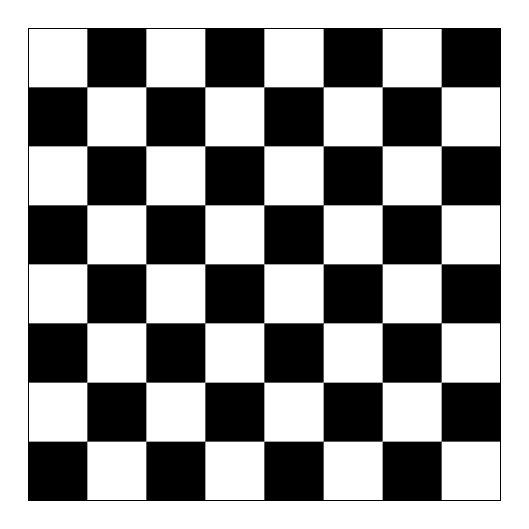
\begin{tikzpicture}[scale=0.75]
			\draw (0,0) rectangle (8,8);
			\foreach \y in {0,2,...,6}{
				\foreach \x in {0,2,...,6}{
					\fill (\x,\y) rectangle (1+\x,1+\y) rectangle (2+\x,2+\y);}}
		\end{tikzpicture}
		\vspace*{-5pt}
	\end{figure}
	Tóm lại ta phủ kín được bảng bằng các hình chữ $T$ khi và chỉ khi $n$ chia hết cho $4$.
	\vskip 0.1cm
	{\bf\color{cackithi} OC$\pmb{27.}$} Giả sử rằng các số thực $a$ và $b$ thỏa mãn
	\begin{align*}
		ab+ \sqrt{ab+1} +\sqrt{a^2+b}\ \sqrt{b^2+a}=0.
	\end{align*}
	Tìm giá trị của biểu thức
	\begin{align*}
		S=a\sqrt{b^2+a} + b\sqrt{a^2+b}.
	\end{align*}
	\textit{\textit{Lời giải}.} Từ đẳng thức trong bài, chuyển vế và bình phương hai vế ta có
	\begin{align*}
		& \ ab+ \sqrt{a^2+b} \sqrt{b^2+a} = -\sqrt{ab+1} \\
		\Rightarrow\  &	a^2b^2 + 2ab\sqrt{a^2+b} \sqrt{b^2+a} \\
		&+ (a^2+b)(b^2+a) = ab+1\\
		\Leftrightarrow\  &	(a^2b^2+a^3) + 2ab\sqrt{a^2+b} \sqrt{b^2+a} \\
		&+ (b^3+a^2b^2) = 1\\
		\Leftrightarrow\ 	& (a\sqrt{b^2+a} + b\sqrt{a^2+b})^2 = 1.
	\end{align*}
	Ta nhận được $S=\pm 1.$ Ta sẽ chứng minh $S$ luôn dương. Thực vậy, từ giả thiết ta có
	\begin{align*}
		ab= -\sqrt{ab+1} -\sqrt{a^2+b} \sqrt{b^2+a} <0.
	\end{align*}
	Không mất tổng quát, ta có thể giả sử \linebreak $a>0>b.$ Khi đó, do $a>\sqrt{a^2+b},$ ta có
	\begin{align*}
		S= a( \sqrt{b^2+a} +b)- b(a- \sqrt{a^2+b})>0.
	\end{align*} 
	Do đó  $S=1$.
	\vskip 0.1cm
	Trong phần cuối của chuyên mục kỳ này, chúng tôi sẽ giới thiệu với bạn đọc ba bài toán trong kỳ thi Olympic Toán học trẻ khối Pháp ngữ năm $2022$. Các bài toán này phù hợp với trình độ học sinh năm cuối cấp Trung học cơ sở.
	\vskip 0.1cm
	{\bf\color{cackithi} OC$\pmb{34.}$} Tìm tất cả các số nguyên dương $n$ sao cho $ \lfloor \sqrt{n}\rfloor $ là ước của $n.$ 
	\vskip 0.1cm
	\textit{Chú ý}: $ \lfloor x \rfloor $ ký hiệu phần nguyên của một số thực $x,$ được định nghĩa là số nguyên lớn nhất nhỏ hơn hoặc bằng $x.$ Ví dụ: $ \lfloor 1.4 \rfloor =1$, $ \lfloor 2 \rfloor=2,$ và  $ \lfloor 2.9 \rfloor= 2.$  
	\vskip 0.1cm
	{\bf\color{cackithi} OC$\pmb{35.}$} Cho một bảng ô vuông cỡ $n \times n$ với $n\ge 1$. Aya muốn tô màu  $k$ ô của bảng  sao cho chỉ có duy nhất một cách để đặt  $n$ đồng xu trên các ô vuông được tô màu sao cho không có hai đồng xu nào nằm trên cùng một hàng hoặc cột. Hỏi giá trị tối đa có thể của $k$  là bao nhiêu?
	\vskip 0.1cm
	{\bf\color{cackithi} OC$\pmb{36.}$} Cho tam giác $ABC$ và $D$ là giao điểm của đường phân giác của góc $\angle BAC$ và đường trung trực của cạnh $AC$. Đường thẳng  đi qua $B$ và song song với $AC$, cắt đường thẳng $AD$ tại $X$. Đường thẳng đi qua $B$ và song song với $CX$, cắt đường thẳng $AC$ tại $Y$. Đường tròn ngoại tiếp tam giác $ABY$ cắt đường thẳng $BX$ tại $E.$ Chứng minh rằng ba điểm $C$ , $D$ và $E$ thẳng hàng.
\end{multicols}